\section{Verifier}
Il Verifier è un ente che offre dei servizi. Nel nostro esempio è un CAF che offre servizi come la richiesta ISEE.\\
Per accedere a questi servizi la connessione viene effettuata tramite la presentazione di una credenziale di tipo PID.
\subsection{Home}
Per accedere ai servizi offerti bisogna prima effettuare la presentazione di una PID ed effettuare una connessione al verifier.
\begin{center}
    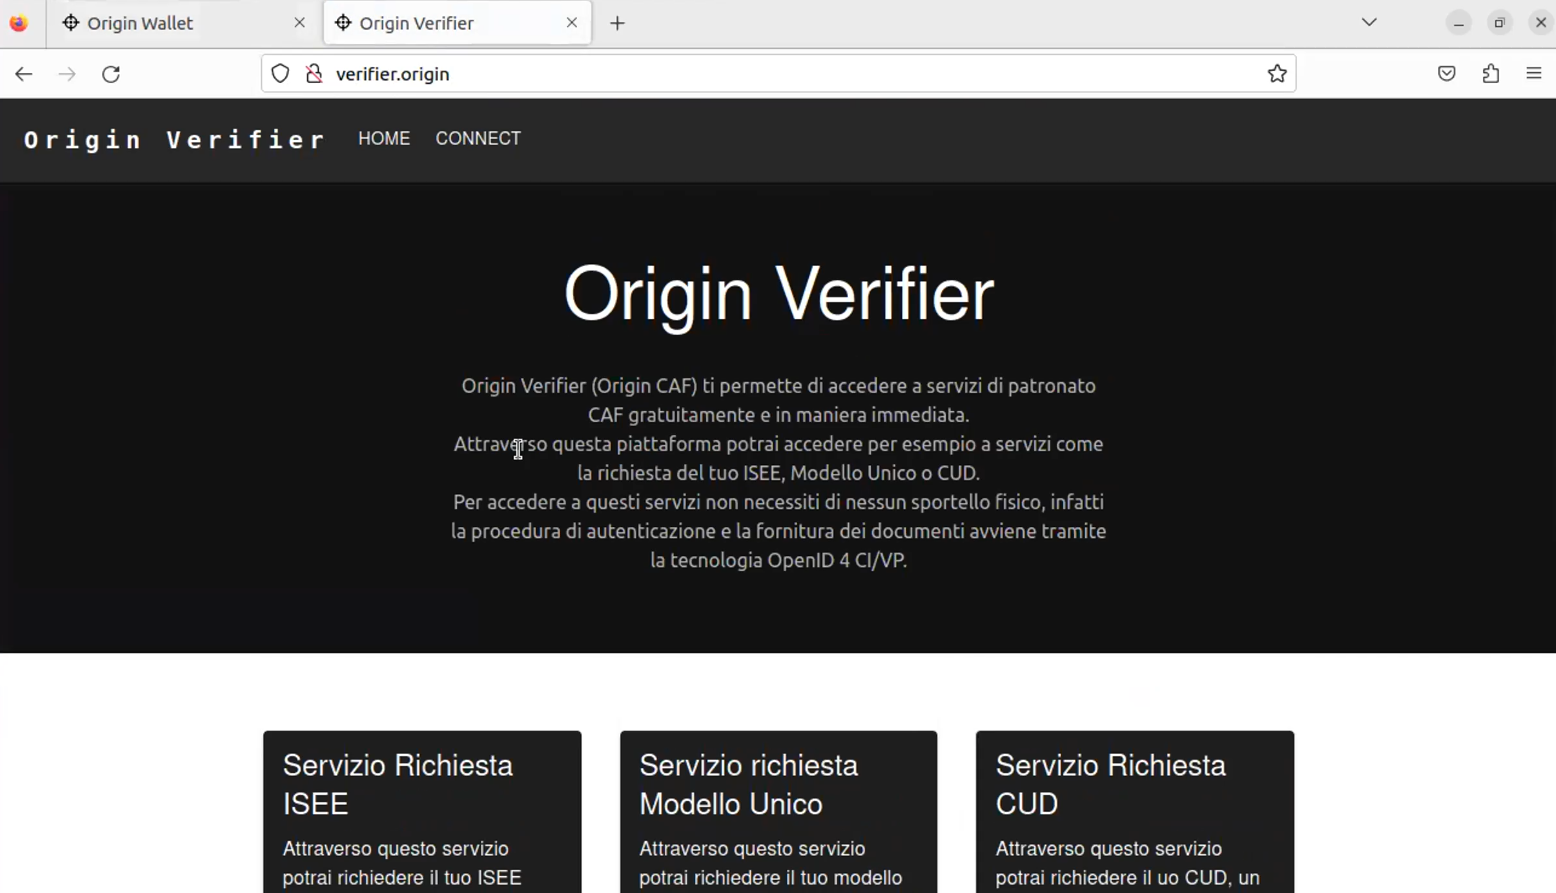
\includegraphics[scale = 0.2]{./res/img/verifier/new/verifier_connect.png}
\end{center}

\subsection{Connessione}
Per accedere ai servizi bisogna effettuare una presentazione di credenziale di tipo PID. La presentazione si può effettuare in modo cross device, inquadrando il qr code, oppure same device, premendo sui pulsanti. Successivamente si verrà reindirizzati al wallet, per continuare la presentazione.
\begin{center}
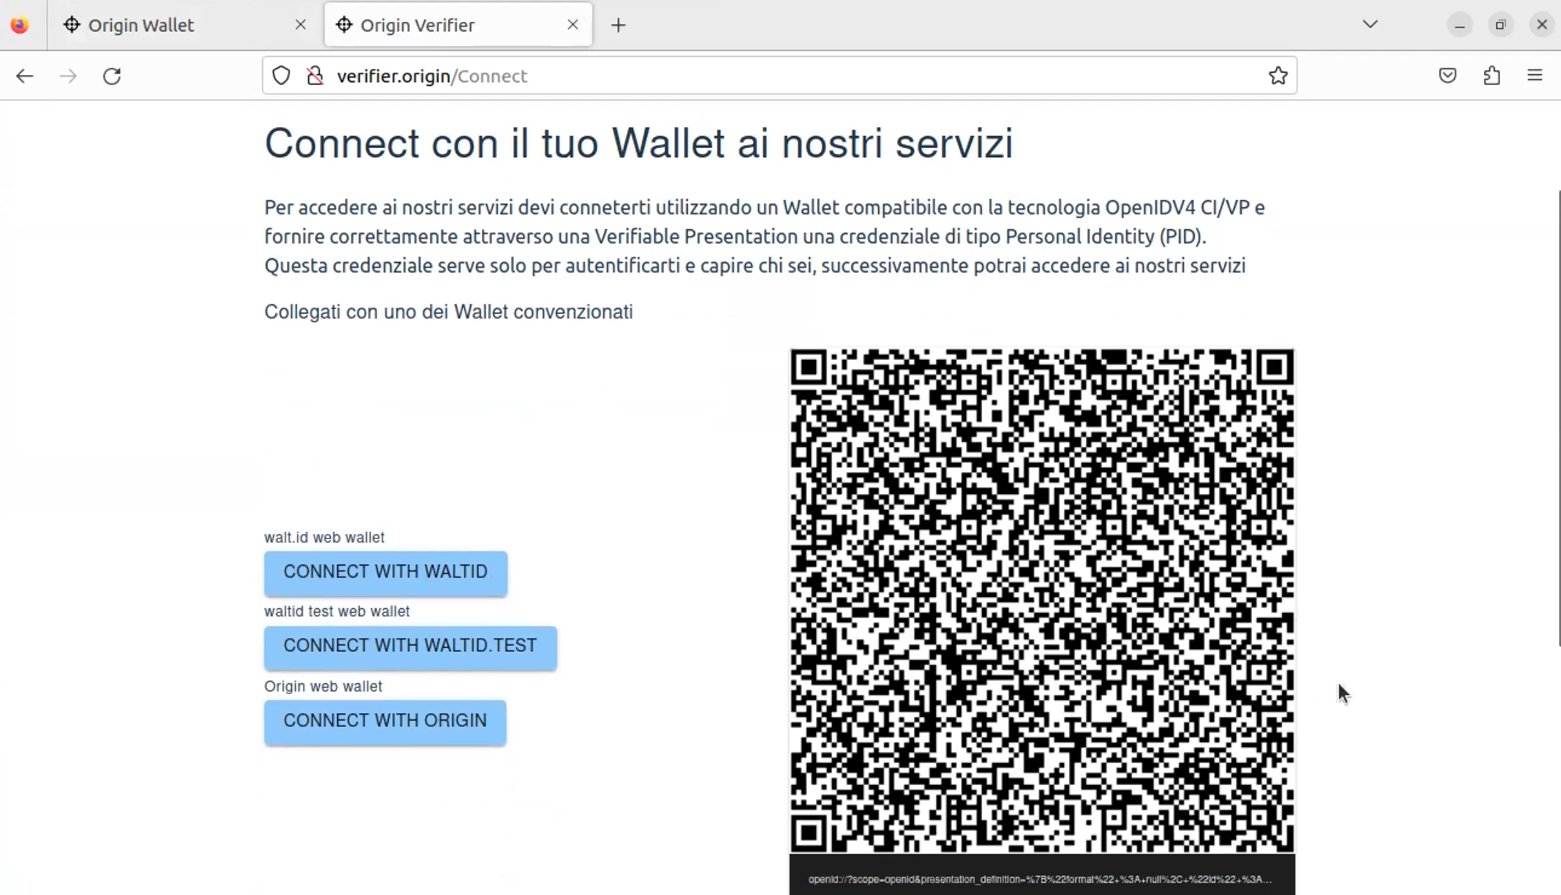
\includegraphics[scale = 0.2]{./res/img/verifier/new/verifier_qr.png}
\end{center}

\subsection{Approvazione presentazione}
Una volta completato da wallet la presentazione di credenziale, si può accettare la presentazione. In particolare si possono visualizzare altri dettagli, come le policy rispettate e l'esito della presentazione.
\begin{center}
    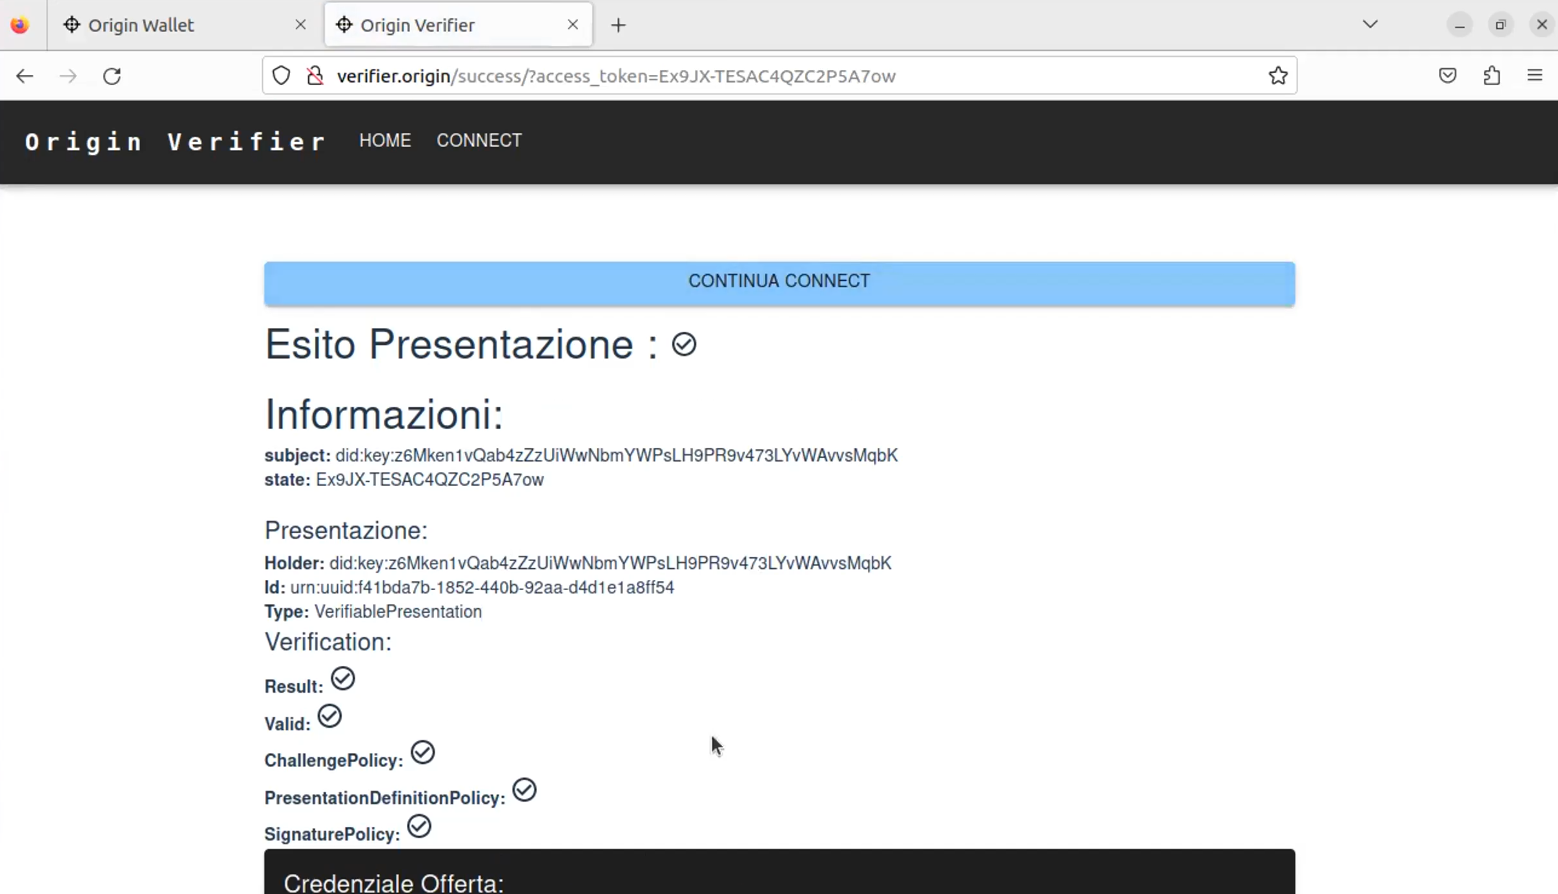
\includegraphics[scale = 0.2]{./res/img/verifier/new/verifier_after_presentation.png}
\end{center}
\subsection{Accesso ai servizi}
Se dalla schermata "Home" provassimo ad accedere ad un servizio offerto da verifier come in questo caso Servizio isee e l'utente non avesse ancora eseguito la connessione al Wallet e verificato la credenziale necessaria per accedervi, verrà mostrato a schermo un messaggio di errore che cita l'invalidità del token.

\begin{center}
    
    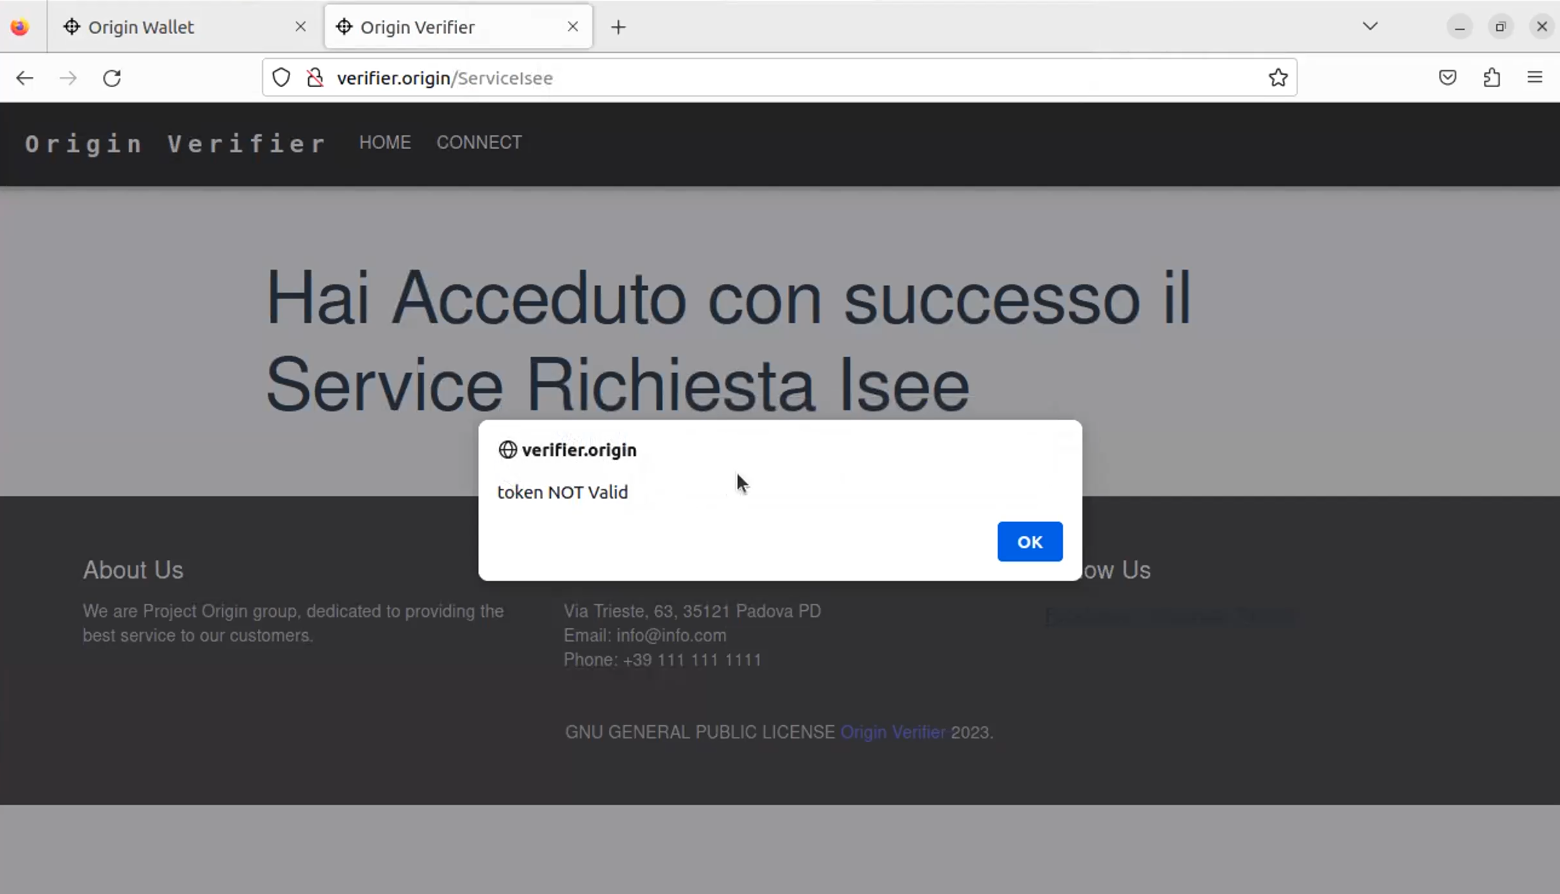
\includegraphics[scale = 0.2]{./res/img/verifier/new/verifier_token_not_valid.png}
\end{center}

Se l'utente avesse completato la  connessione descritta nella sezione precedente può accedere al "Servizio isee" offerto avendo un messaggio di corretto token a disposizione e accedendo correttamente al servizio.\\

\begin{center}
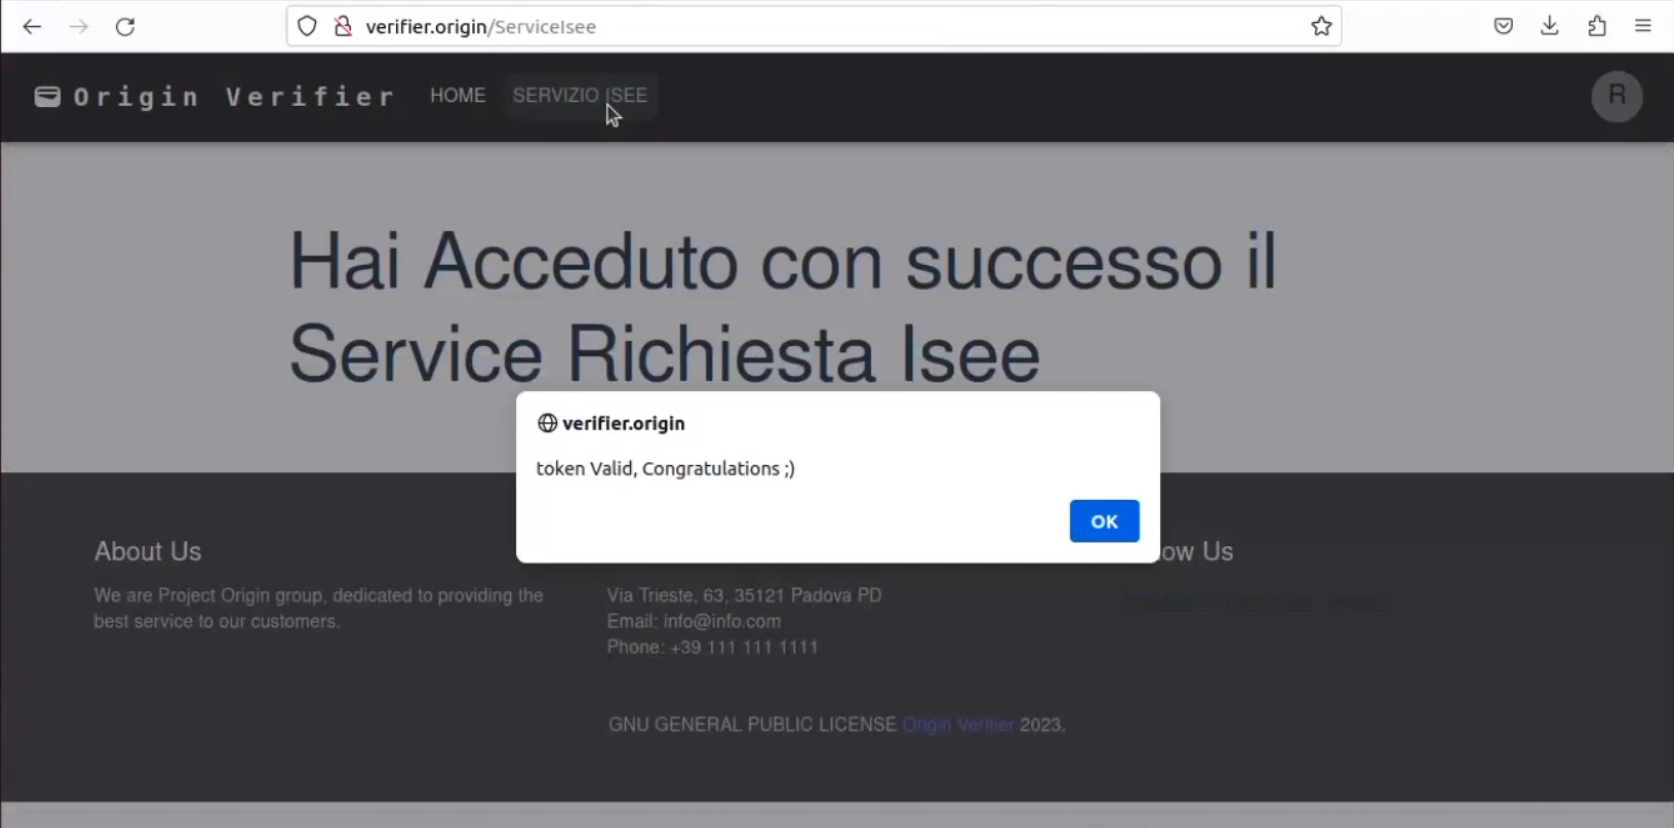
\includegraphics[scale = 0.2]{./res/img/verifier/new/tokenvalido.png}
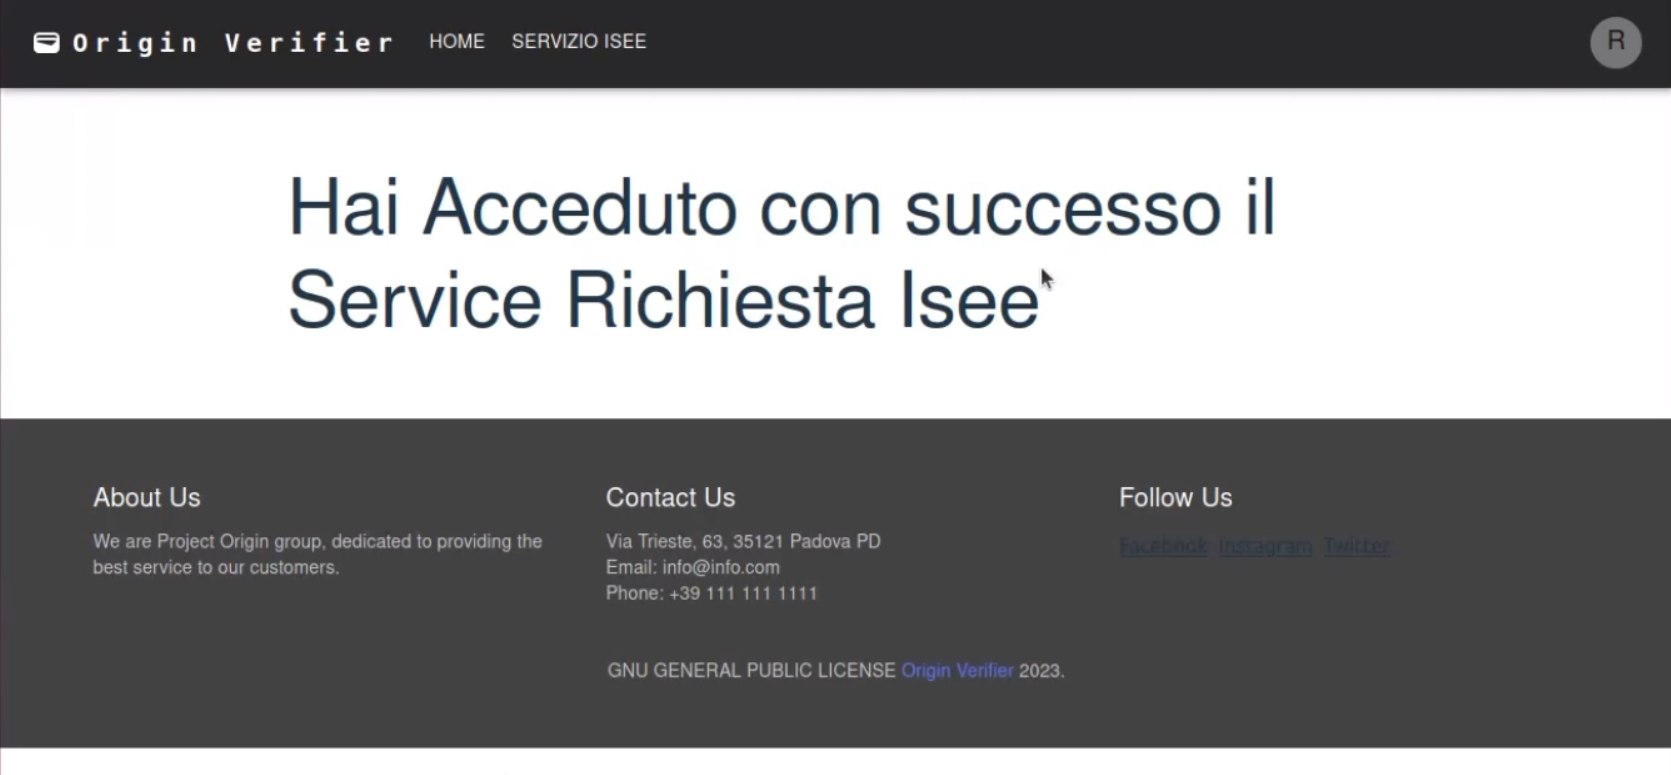
\includegraphics[scale = 0.2]{./res/img/verifier/accessoservizio.png}
\end{center}
